\begin{section}{The Irrationality of $\sqrt{2}$}

In this section we will prove one of the oldest and most important theorems in mathematics: $\sqrt{2}$ is irrational (see Theorem~\ref{thm:sqrt2}). First, we need to know what this means.

\begin{definition}
Let $r\in\mathbb{R}$.
\begin{enumerate}[label=\textrm{(\alph*)}]
\item We say that $r$ is \textbf{rational} if and only if $r=\frac{m}{n}$, where $m,n\in\mathbb{Z}$ and $n\neq 0$.
\item In contrast, we say that $r$ is \textbf{irrational} if and only if it is not rational.
\end{enumerate} 
\end{definition}

The Pythagoreans were an ancient secret society that followed their spiritual leader: Pythagoras of Samos (c.\ 570--495 BCE). The Pythagoreans believed that the way to spiritual fulfillment and to an understanding of the universe was through the study of mathematics. They believed that all of mathematics, music, and astronomy could be described via whole numbers and their ratios. In modern mathematical terms they believed that all numbers are rational. Attributed to Pythagoras is the saying, ``Beatitude is the knowledge of the perfection of the numbers of the soul.'' And their motto was ``All is number.''

Thus they were stunned when one of their own---Hippasus of Metapontum (c.\ 5th century BCE)---discovered that the side and the diagonal of a square are incommensurable. That is, the ratio of the length of the diagonal to the length of the side is irrational. Indeed, if the side of the square has length $a$, then the diagonal will have length $a\sqrt{2}$; the ratio is $\sqrt{2}$ (see Figure~\ref{fig:square}).

\begin{figure}[ht]
\begin{center}
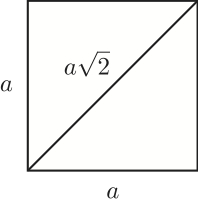
\includegraphics{square.png}
\end{center}
\vspace{-.5cm}
\caption{The side and diagonal of a square are incommensurable.}
\label{fig:square}
\end{figure}

%The following lemma is useful.
%
%\begin{lemma}\label{lem:n^2 even implies n even}
%Let $n\in\mathbb{Z}$. If $n^2$ is even, then $n$ is even.\footnote{Notice that this lemma is the converse of Theorem~\ref{thm:n even implies n^2 even}.}
%\end{lemma}

\begin{theorem}\label{thm:sqrt2}
The real number $\sqrt{2}$ is irrational.\footnote{\emph{Hint:} Use a proof by contradiction.  That is, suppose that there exist $m,n\in\mathbb{Z}$ such that $n\ne 0$ and $\sqrt{2}=\frac{m}{n}$. We may assume that $m$ and $n$ are relatively prime; otherwise, we could cancel common factors. Next, square both sides and solve for $m^2$. How many factors of 2 are on each side of this equation according to the Fundamental Theorem of Arithmetic? Don't actually try to find the exact number of 2's, but rather see if you can figure out if there is an odd or even number of 2's on each side.}
\end{theorem}

As one might expect, the Pythagoreans were unhappy with this discovery. Legend says that Hippasus was expelled from the Pythagoreans and was perhaps drowned at sea. Ironically, this result, which angered the Pythagoreans so much, is probably their greatest contribution to mathematics: the discovery of irrational numbers.

See if you can generalize the technique in the proof of Theorem~\ref{thm:sqrt2} to prove the next two theorems.

\begin{theorem}\label{thm:sqrtp}
Let $p$ be a prime number.  Then $\sqrt{p}$ is irrational.
\end{theorem}

\begin{theorem}\label{thm:sqrt(pq)}
Let $p$ and $q$ be distinct primes.  Then $\sqrt{pq}$ is irrational.
\end{theorem}

\begin{problem}
State a generalization of Theorem~\ref{thm:sqrt(pq)} and briefly describe how its proof would go.  Be as general as possible.
\end{problem}

It is important to point out that not every positive irrational number is equal to the square root of some natural number.  For example, $\pi$ is irrational, but is not equal to the square root of a natural number. It is also worth pointing out that our approach for proving that $\sqrt{2}$ was irrational was not the most efficient.  However, our technique was easy to generalize to handle results like Theorem~\ref{thm:sqrtp}.

\end{section}
